\documentclass[11pt]{scrartcl}
\usepackage[sexy]{../../../evan}
\usepackage{graphicx}

\definecolor{dg}{RGB}{2,101,15}
\newtheoremstyle{dotlessP}{}{}{}{}{\color{dg}\bfseries}{}{ }{}
\theoremstyle{dotlessP}
\newtheorem{property}[theorem]{Property}

\newtheoremstyle{dotlessN}{}{}{}{}{\color{teal}\bfseries}{}{ }{}
\theoremstyle{dotlessN}
\newtheorem{notation}[theorem]{Notation}
% Shortcuts
\DeclarePairedDelimiter\ceil{\lceil}{\rceil} % ceil function

\DeclarePairedDelimiter\paren{(}{)} % parenthesis

\newcommand{\df}{\displaystyle\frac} % displaystyle fraction
\newcommand{\qeq}{\overset{?}{=}} % questionable equality

\newcommand{\Mod}[1]{\;\mathrm{mod}\; #1} % modulo operator

\newcommand{\comp}{\circ} % composition

% Text Modifiers
\newcommand{\tbf}{\textbf}
\newcommand{\tit}{\textit}

% Sets
\DeclarePairedDelimiter\set{\{}{\}}
\newcommand{\unite}{\cup}
\newcommand{\inter}{\cap}

\newcommand{\reals}{\mathbb{R}} % real numbers: textbook is Z^+ and 0
\newcommand{\ints}{\mathbb{Z}}
\newcommand{\nats}{\mathbb{N}}
\newcommand{\complex}{\mathbb{C}}
\newcommand{\tots}{\mathbb{Q}}

\newcommand{\degree}{^\circ}

% Counting
\newcommand\perm[2][^n]{\prescript{#1\mkern-2.5mu}{}P_{#2}}
\newcommand\comb[2][^n]{\prescript{#1\mkern-0.5mu}{}C_{#2}}

% Relations
\newcommand{\rel}{\mathcal{R}} % relation

\setlength\parindent{0pt}

% Directed Graphs
\usetikzlibrary{arrows}
\tikzset{vertex/.style = {shape=circle,draw,minimum size=2em}}
\tikzset{svertex/.style = {shape=circle,draw,minimum size=.05em,font=\tiny}}
\tikzset{edge/.style = {->,> = latex'}}
\tikzset{dedge/.style = {-> = latex'}}
\tikzset{dot/.style={inner sep=1.5pt,circle,draw,fill}}


% Contradiction
\newcommand{\contradiction}{{\hbox{%
    \setbox0=\hbox{$\mkern-3mu\times\mkern-3mu$}%
    \setbox1=\hbox to0pt{\hss$\times$\hss}%
    \copy0\raisebox{0.5\wd0}{\copy1}\raisebox{-0.5\wd0}{\box1}\box0
}}}

\newcommand{\xxhash}[2]{\rotatebox[origin=c]{#2}{$#1\parallel$}}

\title{CS 120: Intro to Algorithms and their Limitations}
\subtitle{PSet 2}
\author{Denny Cao}
\date{\today}
%++++++++++++++++++++++++++++++++++++++++
% title stuff
\usepackage{titling}
\renewcommand\maketitlehooka{\null\mbox{}\vfill}
\renewcommand\maketitlehookd{\vfill\null}
\makeatletter
\renewcommand{\maketitle}{\bgroup\setlength{\parindent}{0pt}
	\begin{flushleft}
		\large\textbf{\@title} \\ \vskip 0.2cm
		\begingroup
		\fontsize{14pt}{12pt}\selectfont
		\title
		\\
		Problem Set 2
		\endgroup \vskip 0.3cm
		Due: September 27, 2023 11:59pm \hfill\rlap{}\textbf{Denny Cao} \\ \vskip 0.1cm
		\hrulefill
	\end{flushleft}\egroup
}
\makeatother

\renewcommand{\theques}{\thesection.\alph{ques}} % Change subtheo counter for alpha output
\declaretheorem[style=basehead,name=Answer,sibling=theorem]{ans}
\renewcommand{\theans}{\thesection.\alph{ans}}
\begin{document}
\maketitle
\pagestyle{plain}
\textbf{Collaborators:}

\textbf{No. of late days used on previous psets:} 0

\textbf{No. of late days used after including this pset:} 1
\section{Reductions}
\begin{enumerate}[(a)]
	\item 
	\begin{proof} \

		We first describe the reduction algorithm.
		\begin{itemize}
			\item Preprocess an array by converting the Cartesian coordinates to polar coordinates, and store $\theta$ as the key and $(r,(x,y))$ as the value. Our array will contain $(\texttt{key}, \texttt{value})$ pairs in the form $(\theta_i, (r_i, (x_i, y_i))$, for all $i \in \set{0,1,\dots, n-1}$, where $(x_i,y_i)$ represents the $i $th coordinate point in the input and $(\theta_i, r_i)$ represents the $i$th coordinate point in the input in polar coordinates.
			\item Sort this array by $K_i$, the angle of the coordinate points in polar form to create a sorted array $S$ by an oracle call to \texttt{Sorting}.
			\item Given $S$, for each pair of adjacent elements $(K_i', V_i') = (\theta_i', (r_i', (x_i', y_i')))$ and $(K_{i+1}', V_{i+1}') = (\theta_{i+1}', (r_{i+1}', (x_{i+1}', y_{i+1}')))$, determine the area of the triangle formed by the two points and the origin at $(0,0)$ by using Heron's Formula and then add it to a variable \texttt{area}: 
	\begin{itemize}
		\item Let $a = r_i', b = r_{i+1}', c = \sqrt{(x_{i+1}'- x_{i}')^2 + (y_{i+1}' - y_{i}' )^2}$.
		\item Let $s = \displaystyle\frac{a+b+c}{2}$.
		\item The area of the triangle is then $\sqrt{s(s-a)(s-b)(s-c)}$.
		\item For $(K_{n-1}', V_{n-1}')$, the adjacent element will be the first element,  $(K_{0}', V_0')$.
	\end{itemize}
\item Return \texttt{area}.
	\end{itemize}
	We now want to prove our reduction algorithm:
	\begin{enumerate}[1.]
		\item has the desired runtime and call size to the \texttt{Sorting} oracle, and
		\item is correct.
	\end{enumerate}
	\begin{itemize}
		\item Forming an array in the first step takes time $O(n)$, as by our assumption, converting into polar coordinates is constant time, and thus there are $O(1)$ operations for each point in the input of size  $n$. Computing basic operations on adjacent elements in the array will take $O(n)$, as there are $O(1)$ operations performed for each of the $n$ elements in the array. Adding the area of the triangle to \texttt{area} will also be a basic operation, taking time $O(1)$, and thus with $n$ areas, will take $O(n)$. Thus, the total time taken by the reduction is $O(n)$. Also, the array passed to \texttt{Sorting} has size $n$, as claimed and the oracle is only called once.
		\item All convex polygons with $n$ sides can be constructed by $n$ triangles using adjacent pairs of vertices and a point in the interior of the polygon as vertices of each triangle. The sum of the area of the triangles will thus be the area of the convex polygon. Our reduction algorithm sorts by $\theta$ in order to obtain adjacent vertices and then obtains the area of the triangles using the origin, $(0,0)$ as the third point which the computational problem states is in the interior of the convex polygon. It then sums all triangle areas together and returns the sum, which is the area of the convex polygon. Thus, our algorithm is correct.
	\end{itemize}
	We have shown that $\texttt{AreaOfConvexPolygon}\leq_{O(n),n}\texttt{Sorting}$ and that the reduction is correct.
	\end{proof}
\item
	\begin{proof}
		We have shown an $O(n)$-time algorithm for \texttt{AreaOfConvexPolygon} that makes one call to the \texttt{Sorting} oracle on an array of size $n$. Thus by Lemma 3 (Lecture 3: Reductions), 
\[
		\text{Time}_{\texttt{AreaOfConvexPolygon}}(n) \leq O(n) + \text{Time}_{\texttt{Sorting}}(n)
\]
Let the \texttt{Sorting} oracle be a sorting function that runs in $O(n\log n)$ time. Thus:
\[
		\text{Time}_{\texttt{AreaOfConvexPolygon}}(n) \leq O(n) + O(n\log n) = O(n\log n)
\] 
Thus, \texttt{AreaOfConvexPolygon} can be solved in time $O(n\log n)$.
	\end{proof}
\item 
\begin{proof}
	Let $\gamma$ be an algorithm that solves  $\Gamma$ and let $\pi$ be an algorithm that solves $\Pi$. As $\Pi$ can be reduced to $\Gamma$, we can view $\gamma$ as the oracle that solves $\Gamma$. Let $\pi$ call $\gamma$. 
\\

	Then, the runtime of $\pi$ can be bounded by the sum of the maximum time for preprocessing and postprocessing for $\gamma$ and the maximum time it takes for all calls of $\gamma$. As each call of $\gamma$ takes time $T(n)$ for an input size $n$ and the greatest input size possible is $h(n)$, then each call of $\gamma$ takes time at most $O(T(h(n)))$. 
	\\

	As $\gamma$ is called at most $k(n)$ times, the maximum time for all calls of $\gamma$ is $O(k(n)T(h(n)))$. As the reduction runs in time at most $g(n)$, then the preprocessing and postprocessing for $\gamma$ takes at most $O(g(n))$ time. Thus, the maximum time it takes for an algorithm $\pi$ to solve $\Pi$ is $O(g(n) + k(n)\cdot T(h(n)))$. It follows that the maximum time it takes for $\Pi$ to be solved if $\Gamma$ can be solved in at most $T(n)$ is $O(g(n) + k(n)\cdot T(h(n)))$.
\end{proof}
\item 
	\
	\begin{proof}
		We first describe the reduction algorithm.
		\begin{itemize}
			\item Preprocess 4 arrays $Q_j, j \in \set*{1,2,3,4}$, where $Q_j$ denotes the array of coordinates in the $j$th quadrant. For each Cartesian coordinate pair,  $(x_i, y_i)$,  $i \in \set*{0,1,\dots, n-1}$, compute the slope $m_i$ between the point and the origin $(0,0)$ by setting $m_i = \displaystyle\frac{y_i}{x_i}$ (if $x = 0$, then the slope will be \texttt{MAX} if $y>0$ and \texttt{MIN} if $y < 0$). We then insert each coordinate pair into its corresponding array in $(\texttt{key}, \texttt{value})$ pairs in the form  $(m_i, (x_i, y_i))$, for all  $i \in \set*{0,1,\dots,n-1}$. If $x_i = 0 \land y > 0$, then insert into  $Q_1$. If $x_i < 0 \land y = 0$, then insert into  $Q_2$. If  $x_i = 0 \land y < 0$, then insert  $Q_3$, $x > 0 \land y = 0$, then insert  $Q_4$.
			\item For each array, sort the array by increasing $m_i$, the slope of the coordinate points by an oracle call to \texttt{Sorting}.
			\item Join the arrays together into an array $S$ in order, with $Q_1$ preceding  $Q_2$ which precedes $Q_3$ which precedes $Q_4$.
			\item Given $S$, for each pair of adjacent elements $(K_i', V_i') = (m_i', (x_i', y_i'))$ and $(K_{i+1}', V_{i+1}') = (m_{i+1}', (x_{i+1}', y_{i+1}'))$, determine the area of the triangle formed by the two points and the origin at $(0,0)$ by using Heron's Formula and then add it to a variable \texttt{area}:
				\begin{itemize}
					\item Let $a = \sqrt{x_i'^2 + y_i'^2}, b = \set*{x_{i+1}'^2 + y_{i+1}'^2}, c = \sqrt{(x_{i+1}' - x_i')^2 + (y_{i+1}' - y_i)^2}$.
					\item Let $s = \displaystyle\frac{a+b+c}{2}$.
					\item The area of the triangle is then  $\sqrt{s(s-a)(s-b)(s-c)}$.
					\item For  $(K_{n-1}', V_{n-1}')$, the adjacent element will be the first element,  $(K_0', V_0')$.
				\end{itemize}
			\item Return \texttt{area}.
		\end{itemize}
		Creating the 4 quadrant arrays takes $O(1)$ time. Iterating through the inputs and getting slope and adding to the respective quadrant array for each input takes $O(1)$ time, resulting in $O(n)$ time. We call the oracle $O(1)$ calls, as we always call it for 4 quadrant arrays. Thus, it runs in $O(n)$. If we take sorting into account, $O(n) + O(n\log n) = O(n\log n)$. The correctness proof is the same as (c).
	\end{proof}
\end{enumerate}
\section{Augmented Binary Search Trees}
\begin{enumerate}[(a)]
	\item The \texttt{select} function has a correctness error. When \texttt{ind} is greater than \texttt{left\_size}, the algorithm checks the right subtree. However, it attempts to find the \texttt{ind} least key on the right subtree, which would imply that the selected key would be the \texttt{ind + left\_size} least key, since all elements on the left subtree are less than the right. The fix is to instead find the \texttt{ind - left\_size} least key on the right, as that would mean the number we selected would be the \texttt{ind} least key.
		\\

		The \texttt{insert} function is too slow. The run time is $O(hn)$, as it traverses to only 1 node in every level, but in each level, it calls \texttt{calculate\_sizes} which has runtime $O(n)$, as it traverses every node in the tree. The fix is to instead of calling \texttt{calculate\_sizes}, setting the current node $k$'s size to  \texttt{k.size = 1 + k.left.size + k.right.size}, and removing \texttt{k.left.size} if \texttt{k.left is None} and removing \texttt{k.right.size} if \texttt{k.right is None}, allowing the calculation of sizes to be done only on the nodes that are affected by the insertion, and in $O(1)$ time for each node. 
		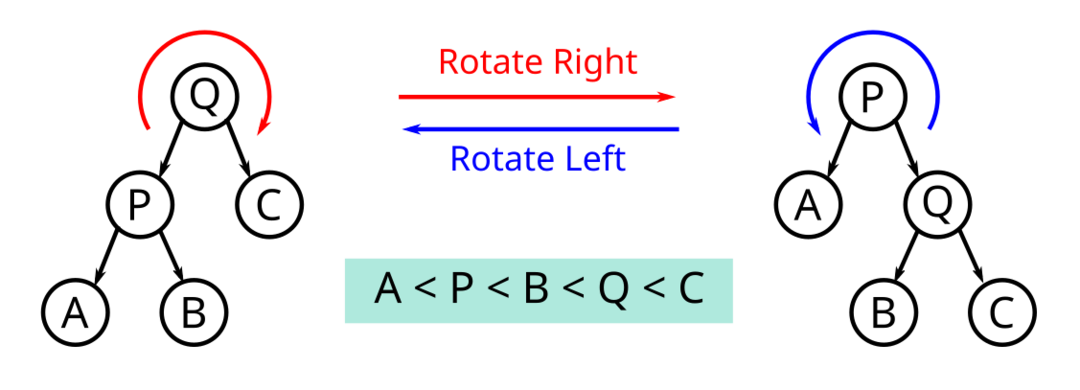
\includegraphics[width=\textwidth]{Tree_rotation}
	\item We use the rotation algorithm for BSTs depicted above and will extend it to size-augmented BSTs.
		\\

		We consider the case of a right rotation. In this case, the rotation can remain the same, but we must change the size attributes of the nodes. Let \texttt{x.size} denote the size of a node $x$. Then, after a right rotation, \texttt{P.size = A.size + B.size + C.size + 2} and \texttt{Q.size = B.size + C.size + 1}. The same argument can be made for the left rotation by interchanging $P$ and $Q$.
		\\
		\begin{claim*}
			The extension of \texttt{rotation} maintains the runtime $O(1)$.
		\end{claim*}
		\begin{proof}
		The extension maintains the runtime $O(1)$, as the rotation itself takes $O(1)$ time, accessing the size attributes of 3 subtrees $A, B, C$  is a basic operation and takes $O(1)$ time, and setting the size attribute for $P$ and $Q$ is a basic operation and takes $O(1)$. Thus, the runtime remains $O(1)$. 
		\end{proof}
		\begin{claim*}
			The new rotation operation preserves the invariant of correct size-augmentations.
		\end{claim*}
		\begin{proof}
		The new rotation operation preserves the invariant of correct size-augmentations, as the subtrees $A, B, C$ are not affected during the rotation, and the size attributes for $A,B,C$ were correct before the rotation, they remain correct after the rotation. If there exists a parent for the node being rotated ($P$ when rotating left, $Q$ when rotating right), no descendants are removed, and thus the size of the parent will be the same and remain correct. The sizes of $P$ and  $Q$ are defined as the sum of the sizes of the children and the node itself, and thus the size of $P$ and $Q$ are also correct.
		\end{proof}
\end{enumerate}
\end{document}
